\newpage
\subsection{Hidden Single}
\label{Hidden Single}
Auch die Technick \textit{Hidden Single} arbeitet wieder mit Kandidatenlisten. Wenn in einer Figur eine Kandidatenliste die Einzige ist, in der eine bestimmte Zahl vorkommt, dann kann diese Zahl direkt in die Zelle eingetragen werden. Wenn in dieser Zelle die Zahl nicht stünde, dann gäbe es in der Figur keine Möglichkeit mehr, dass die Zahl auftaucht und damit wäre die Sudoku Regel verletzt, nach der jede Zahl genau einmal in jeder Figur enthalten sein muss.

\begin{figure}[h]
\begin{center}
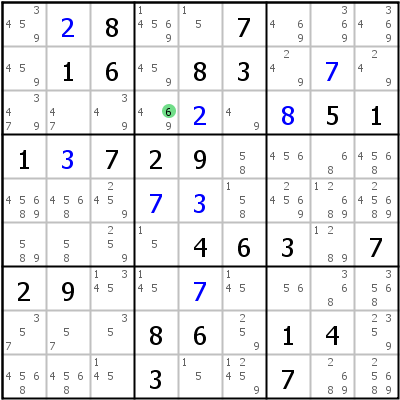
\includegraphics{./img/hidden_single.png}
\caption{Hidden Single}
\end{center}
\end{figure}

\noindent In \textbf{Abbildung 2.5} sieht man, dass die Ziffer 6 in der Zeile 3 nur in z3s1 vorkommen kann. Da in Zeile 3 die Ziffer 6 genau einmal vorkommen kann und sie nur an einer Position in dieser Zeile stehen kann, bleibt keine andere Möglichkeit, als sie dort einzutragen.
